\subsubsection{HOG+SVM}
\paragraph{Lý do sử dụng HOG+SVM cho bài toán\\}
Phương pháp HOG (Histogram of Oriented Gradients) kết hợp với SVM (Support Vector Machines) được chọn để giải quyết bài toán phát hiện người đi bộ với những lý do:
\begin{itemize}[noitemsep, topsep=0pt, leftmargin=1.25em, label={$-$}]
    \item Đơn giản và hiệu quả tính toán: HOG sử dụng tính toán đơn giản, nó chỉ yêu cầu tính gradient của hình ảnh và xây dựng histogram các hướng gradient. Quá trình này có thể thực hiện nhanh chóng trên các hình ảnh tĩnh và không yêu cầu tài nguyên tính toán phức tạp.
    \item Đặc trưng HOG phù hợp cho hình ảnh: HOG nhạy bén với cấu trúc dọc và đặc trưng hình học của người đi bộ, chẳng hạn như cạnh và góc cơ thể vì khả năng trích xuất thông tin hướng và độ lớn của gradient.
    \item SVM là một bộ phân loại mạnh mẽ: SVM là một thuật toán học máy được sử dụng rộng rãi trong việc phân loại và nhận dạng. SVM có khả năng tạo ra một ranh giới quyết định tối ưu giữa các lớp dữ liệu (người đi bộ và không phải người đi bộ). SVM có khả năng xử lý các bài toán phân loại tuyến tính và phi tuyến tính, điều này rất hữu ích trong việc xác định những đặc trưng phức tạp của người đi bộ trong không gian đặc trưng HOG.
    \item Độ ổn định và khả năng tổng quát hóa\cite{reasontousehogsvm}: Phương pháp HOG và SVM có khả năng ổn định và tổng quát hóa tốt đối với các biến đổi trong ánh sáng, môi trường và biến thể về cách thức di chuyển của người đi bộ. Điều này giúp cho phương pháp này có khả năng hoạt động tốt trong các tình huống thực tế.
\end{itemize}
Mặc dù hiện nay phương pháp này không được sử dụng nhiều bời các phương pháp deep learning phát triển rất mạnh mẽ nhờ khả năng học tự động và hiệu suất cao hơn của chúng, nhưng đây vẫn là một phương pháp với thuật toán đơn giản và dễ hiểu được sử dụng để giải quyết bài toán phát hiện đối tượng là người đi bộ.
\paragraph{HOG\\}
HOG (Histogram of Oriented Gradients) là một phương pháp mô tả đặc trưng dùng để biểu diễn hình dạng và diện mạo của một đối tượng trong một hình ảnh. Thuật toán HOG tính toán và biểu thị sự phân bố và hướng của gradient (độ dốc) trong hình ảnh.  

HOG được giới thiệu bởi Navneet Dalal và Bill Triggs vào năm 2005 như một phương pháp hiệu quả để phát hiện đối tượng trong ảnh, đặc biệt là trong bài toán phát hiện người đi bộ.   

Quá trình trích xuất đặc trưng HOG bao gồm các bước chính như sau:
\begin{itemize}[noitemsep, topsep=0pt, leftmargin=1.25em, label={$-$}]
    \item Chia hình ảnh thành các ô (cells): Hình ảnh được chia thành các ô nhỏ, mỗi ô đại diện cho một vùng nhỏ trên hình ảnh.
    \item Tính toán gradient: Gradient của các pixel trong mỗi ô được tính bằng cách sử dụng phương pháp gradient, để xác định độ dốc và hướng của các điểm ảnh. 
    \item Tạo histogram các hướng gradient: Dựa trên gradient, một histogram được tạo ra cho mỗi ô. Histogram này biểu thị phân bố các hướng gradient trong ô đó. 
    \item Chuẩn hóa histogram: Mỗi histogram được chuẩn hóa để giảm ảnh hưởng của ánh sáng và độ tương phản. Thông thường, chuẩn hóa được thực hiện bằng cách chuẩn hóa L2 (Euclidean) của histogram, tức là chuẩn hóa tổng bình phương các giá trị trong histogram về 1.
    \item Kết hợp các vector đặc trưng HOG: Các vector đặc trưng HOG của các ô liền kề được kết hợp thành một vector đặc trưng duy nhất cho toàn bộ hình ảnh. Bước này giúp bao gồm thông tin về sự phân bố của đặc trưng trên cả hình ảnh.
\end{itemize}
\pagebreak
\begin{figure}[h!]
  \centering
  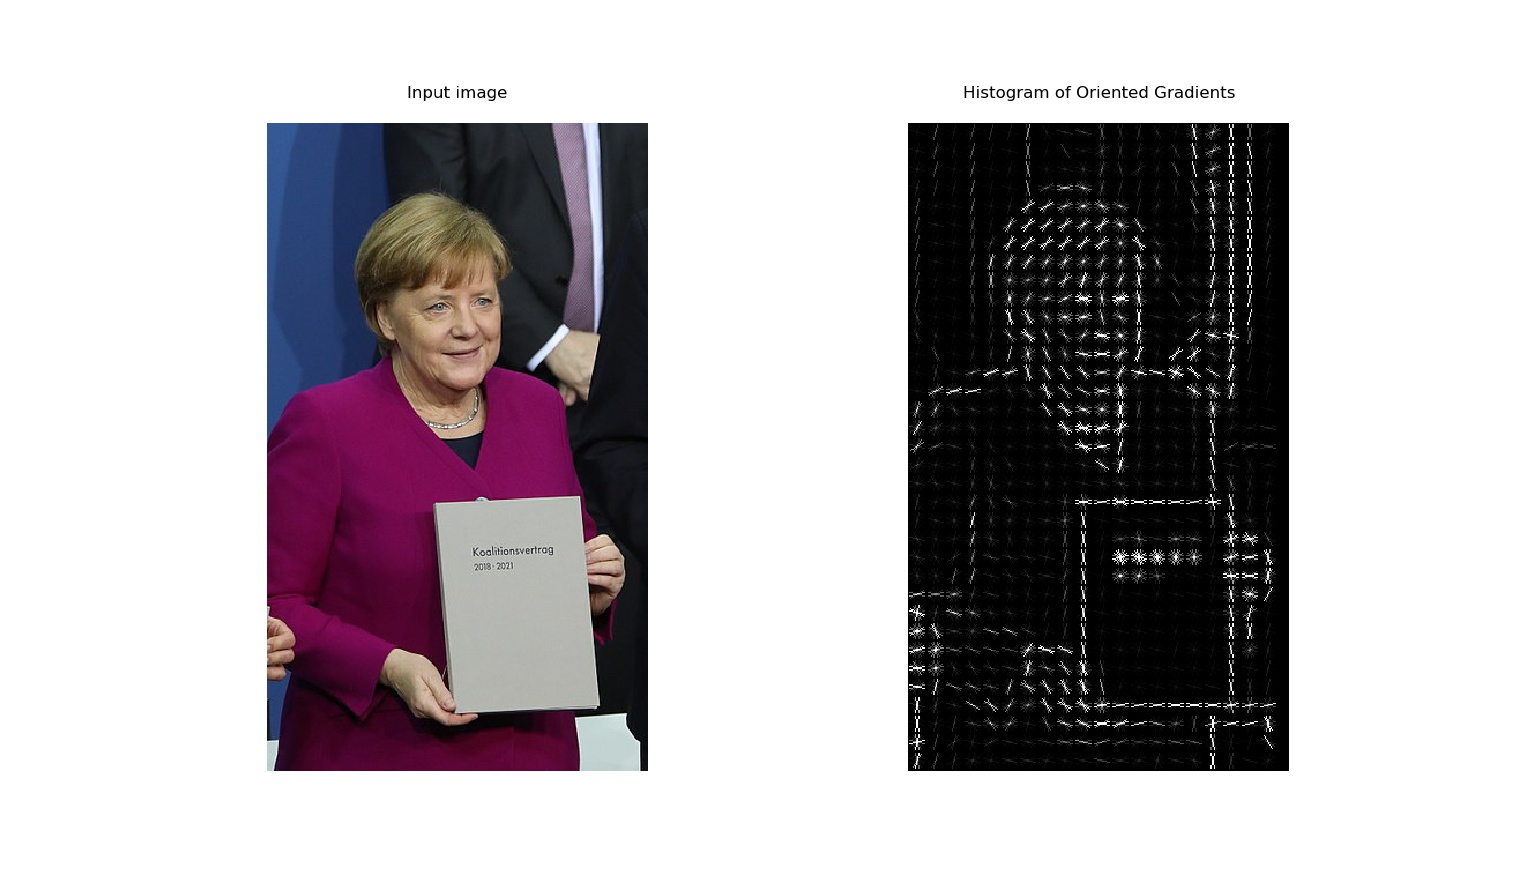
\includegraphics[scale=0.35]{graphics/HOG.jpeg}
  \caption{Kết quả của quá trình trích xuất đặc trưng HOG}
\end{figure}

\paragraph{SVM\\}
Support Vector Machine là một thuật toán máy học có giám sát, sử dụng để phân loại và dự báo. Trong việc phát hiện đối tượng, SVM thường được sử dụng như một bộ phân loại để phân biệt giữa đối tượng cần phát hiện và nền.

SVM hoạt động bằng cách tìm ra siêu phẳng tối ưu (hyper-plane) để phân tách các điểm dữ liệu vào các lớp khác nhau. Nó cố gắng tối ưu hóa khoảng cách giữa hyper-plane và các điểm dữ liệu gần nhất của mỗi lớp. Các điểm dữ liệu nằm trên ranh giới hoặc trong ranh giới được gọi là các vector hỗ trợ (support vectors). SVM có thể xử lý dữ liệu không tách biệt tuyến tính bằng cách sử dụng hàm kernel để biến đổi không gian đầu vào thành không gian đặc trưng có số chiều cao hơn.
\graphicspath{{figures/}}
\begin{figure}[h!]
  \centering
  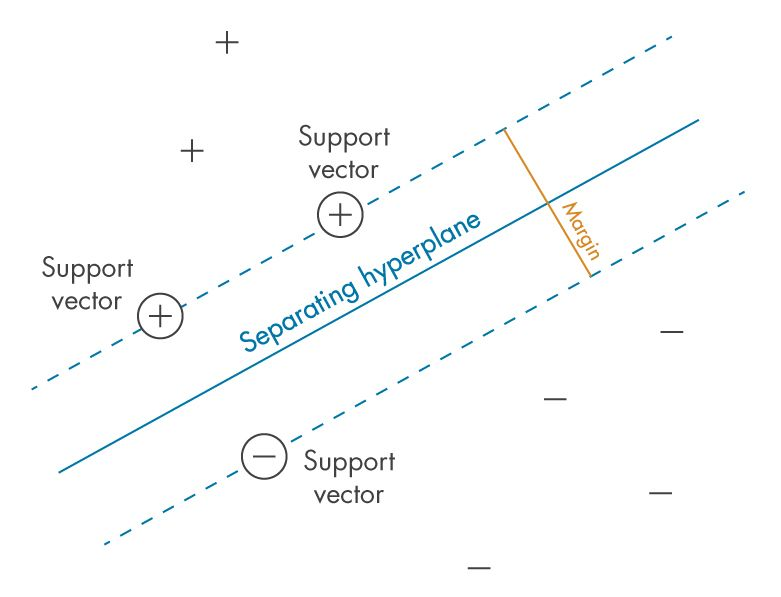
\includegraphics[scale=0.35]{graphics/SVM.jpg}
  \caption{SVM tối ưu hóa khoảng cách giữa hyper-plane và các support vector}
\end{figure}

Các bước chính trong quá trình huấn luyện SVM là:
\begin{itemize}[noitemsep, topsep=0pt, leftmargin=1.25em, label={$-$}]
    \item Xác định đặc trưng: Dữ liệu đầu vào cần được biểu diễn bằng các đặc trưng có ý nghĩa. Các đặc trưng này thường được trích xuất thông qua các phương pháp như HOG, SIFT.
    \item Xây dựng mô hình: Sau khi có các đặc trưng, mô hình SVM được xây dựng bằng việc tìm ra siêu phẳng tốt nhất để phân tách các lớp dữ liệu. Có nhiều loại SVM khác nhau như SVM tuyến tính, SVM hạt nhân (kernel SVM) và SVM đa lớp (multiclass SVM).
    \item Tối ưu hóa: Mục tiêu của SVM là tìm ra hyper-plane tối ưu sao cho khoảng cách (margin) từ siêu phẳng đến các support vectors là lớn nhất. Quá trình này thường được thực hiện bằng cách giải một bài toán tối ưu hóa bậc hai.
    \graphicspath{{figures/}}
    \begin{figure}[h!]
      \centering
      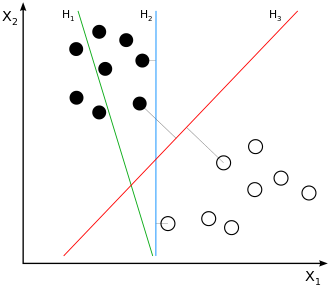
\includegraphics[scale=0.6]{graphics/Svm_separating_hyperplanes.png}
      \caption{H3 là hyper-plane tối ưu với margin tối đa ngăn cách các support vectors}
    \end{figure}
    \item Dự đoán: Sau khi huấn luyện mô hình, SVM có thể được sử dụng để dự đoán lớp của các điểm dữ liệu mới dựa trên vị trí của chúng đối với hyper-plane đã xác định.
\end{itemize}    
Support Vector Machine hiểu một cách đơn giản là một biên giới để chia hai lớp tốt nhất. Đây là một thuật toán học máy mạnh mẽ và đa dụng, một phương pháp hiệu quả cho bài toán phân lớp dữ liệu. SVM cũng có khả năng phân loại tốt trên các tập dữ liệu lớn và ít bị ảnh hưởng bởi nhiễu. Tuy nhiên, nó cũng đòi hỏi tính toán phức tạp và lựa chọn tham số cho phù hợp. Quá trình huấn luyện SVM có thể yêu cầu nhiều tài nguyên tính toán và thời gian, đặc biệt là trên các tập dữ liệu lớn. SVM có các tham số như hàm kernel, thông số đường mềm (soft margin), và hệ số điều chỉnh. Lựa chọn tham số đúng cũng là một yếu tố quan trọng để đạt được hiệu suất tốt của mô hình SVM.